\section{Ejercicio 1}

Para la resolución de este ejercicio se requería generar \emph{n} tareas
bloqueantes con una duración aleatoria de valor $bmin \leq t \leq bmax$. La forma de
lograr esto fue mediante un ciclo que realiza \emph{n} llamados bloqueantes cuya
duración está dictaminada por el siguiente código:

\begin{center}
	\texttt{t = rand() \% (bmax - bmin + 1) + bmin;}
\end{center}

Se utiliza la función \texttt{rand()} habiendo previamente cargado una semilla.
Esto genera un valor $0 \leq r \leq RAND\_MAX$. Para que quede dentro de los
límites definidos con anterioridad, se toma el módulo correspondiente de
\emph{r} sumándole luego \emph{bmin}.

\begin{figure}[ht]
	\begin{center}
		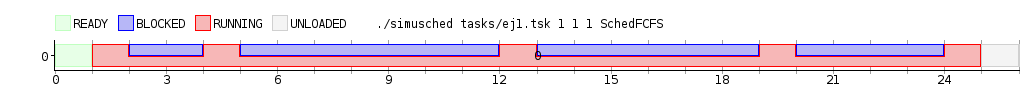
\includegraphics[width=1\columnwidth]{imagenes/ej1.png}
		\caption{\texttt{TaskConsola} corriendo con $n = 4$, $bmin = 2$ y $bmax
		= 7$.}
	\end{center}
\end{figure}

